\subsection{\label{sec:calib.st}Start Counter Calibration and Resolution}

The start counter time-walk calibration took into account the varying geometry of the paddles. Fig.~\ref{fig:calib.st.adcuncor} shows the uncorrected timing difference for paddle 3 (of 24) as a function of \abbr{ADC} while Fig.~\ref{fig:calib.st.adccor} shows the corrected timing. This was done for each paddle and the resulting resolutions can be seen in Fig.~\ref{fig:calib.st.timepion} for pions, Fig.~\ref{fig:calib.st.timeproton} for protons, Fig.~\ref{fig:calib.st.timepion2d} for pions and all paddles, Fig.~\ref{fig:calib.st.timepion.ebeam} for pions a function of beam energy and Fig.~\ref{fig:calib.st.timepion.region} for pions as a function of geometry. The run-by-run resolution can be seen in Fig.~\ref{fig:calib.st.runbyrun}.

% ADC Uncorrected
\begin{figure}[htbp]\begin{center}
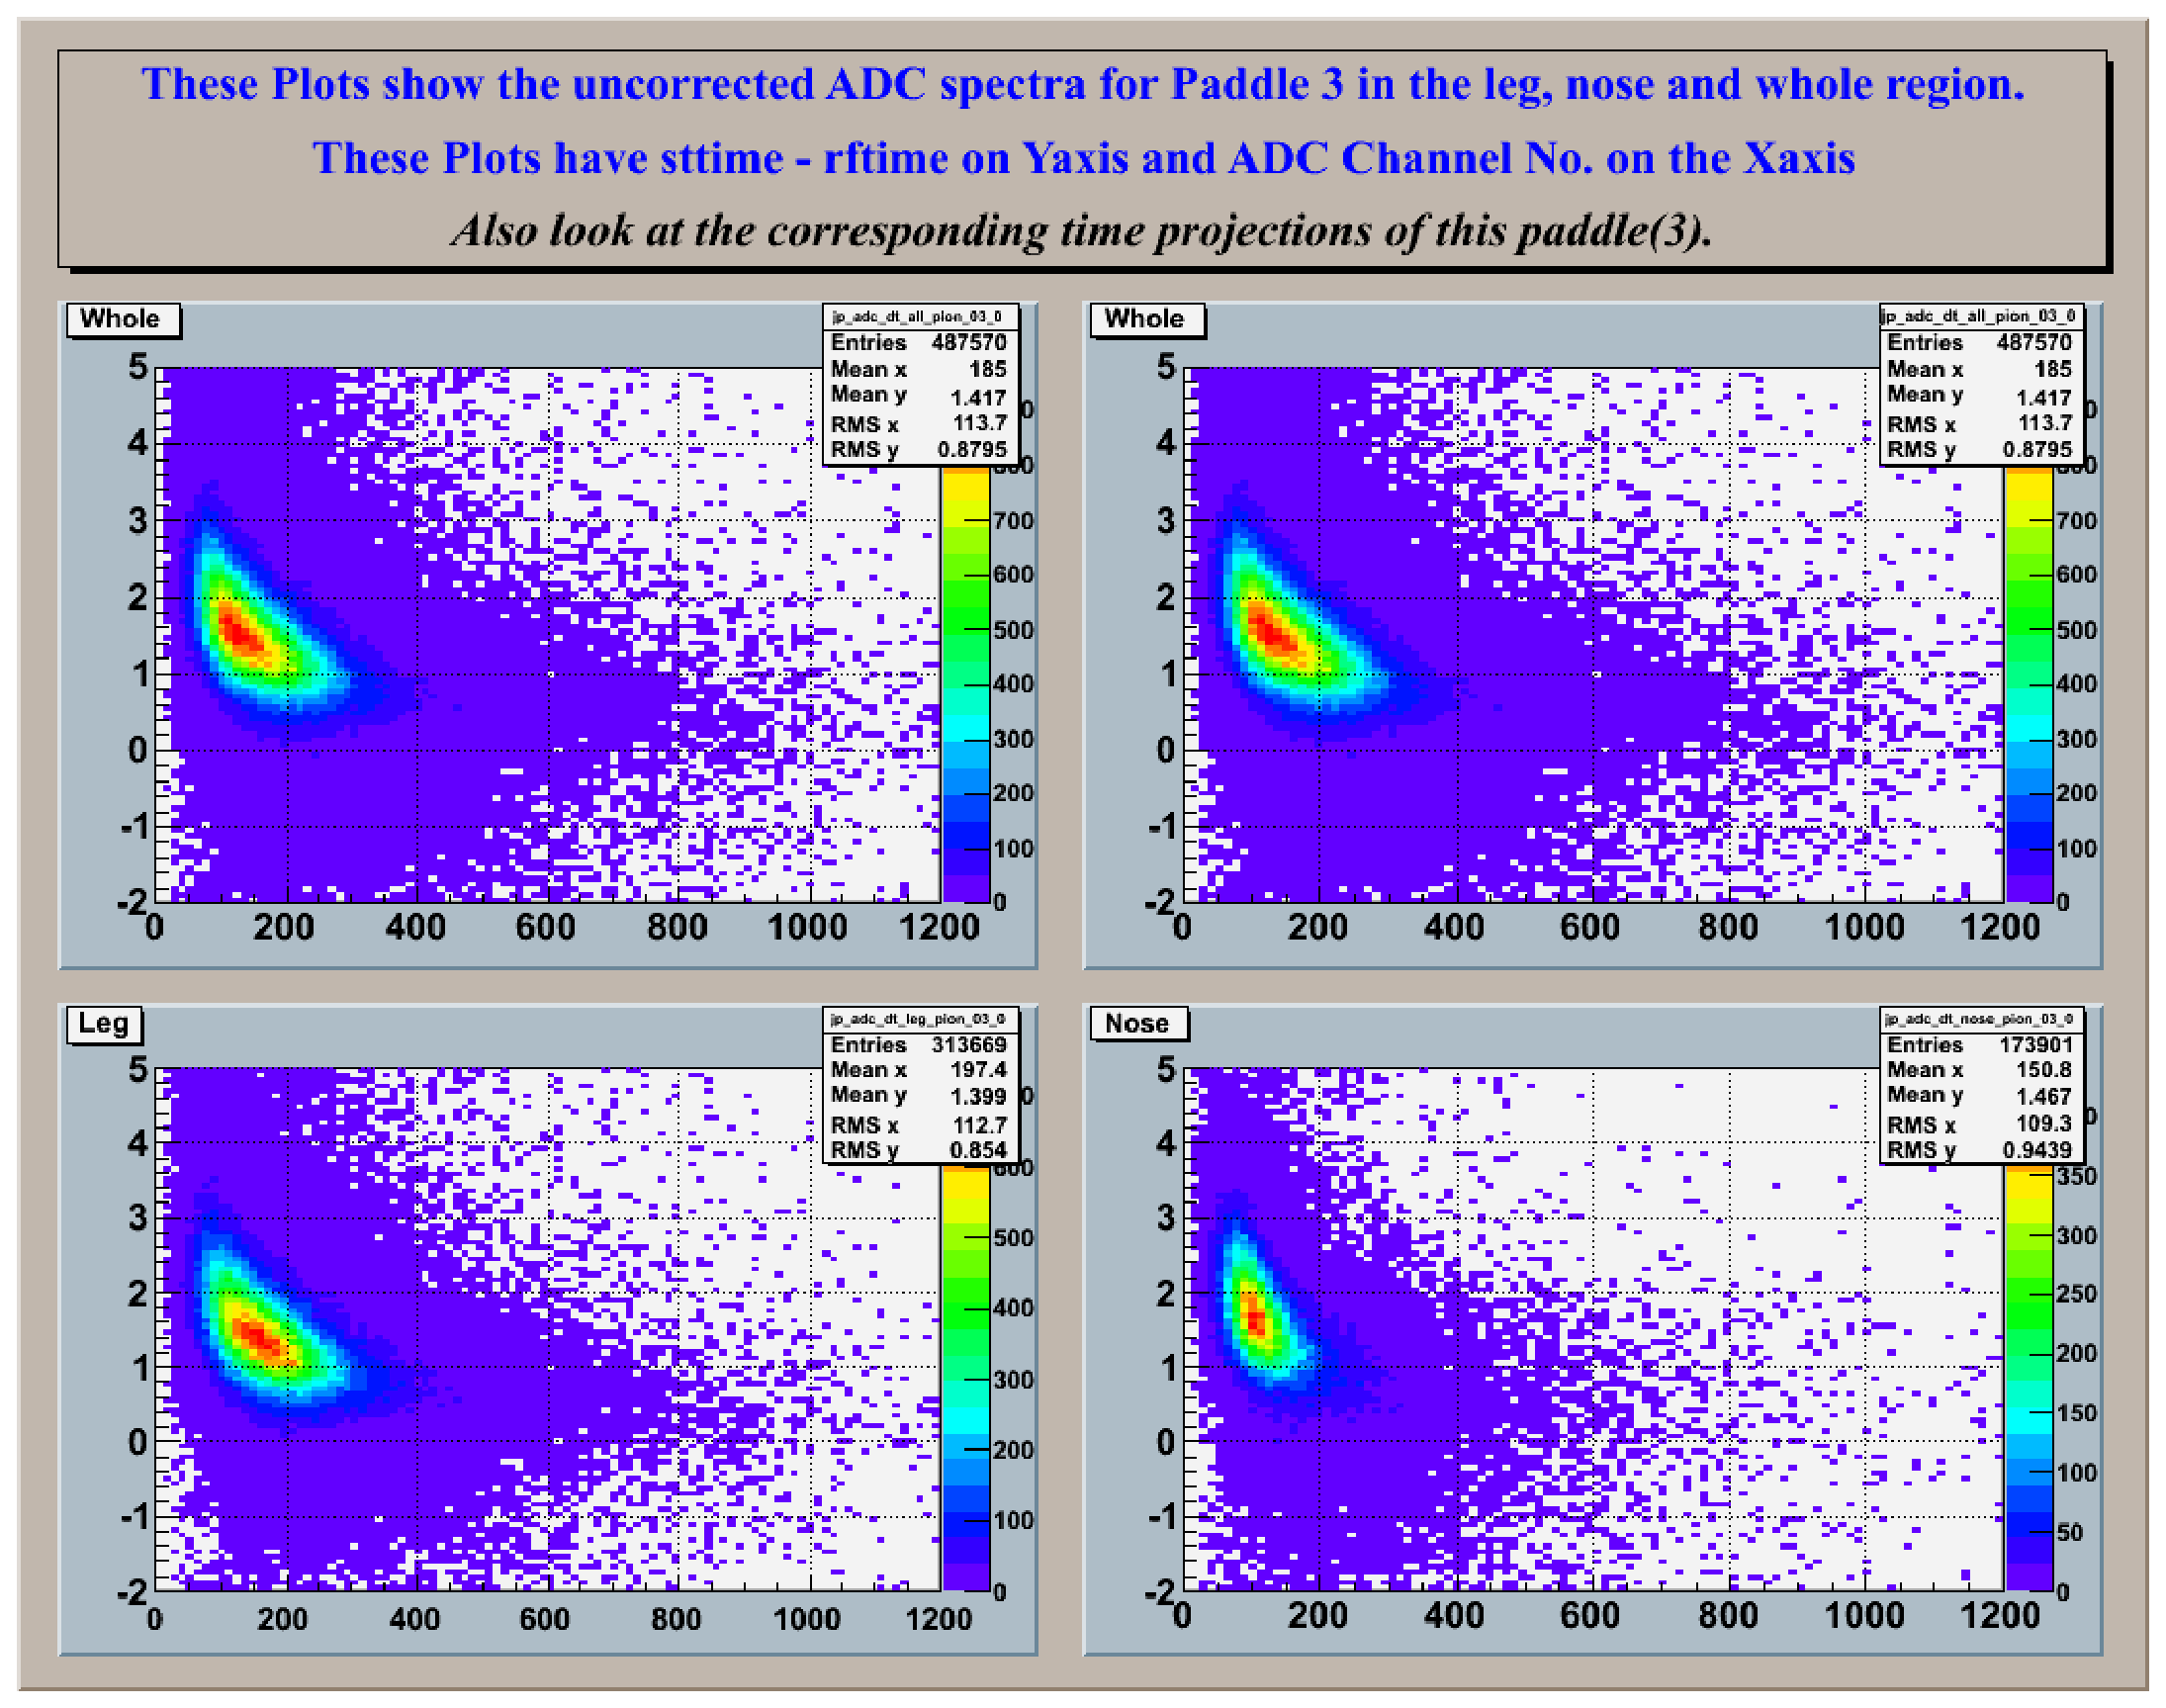
\includegraphics[width=0.65\columnwidth]{figures/calib/st/Uncorrected_adc.eps}
\caption[]{\label{fig:calib.st.adcuncor}}
\end{center}\end{figure}

% ADC Corrected
\begin{figure}[htbp]\begin{center}
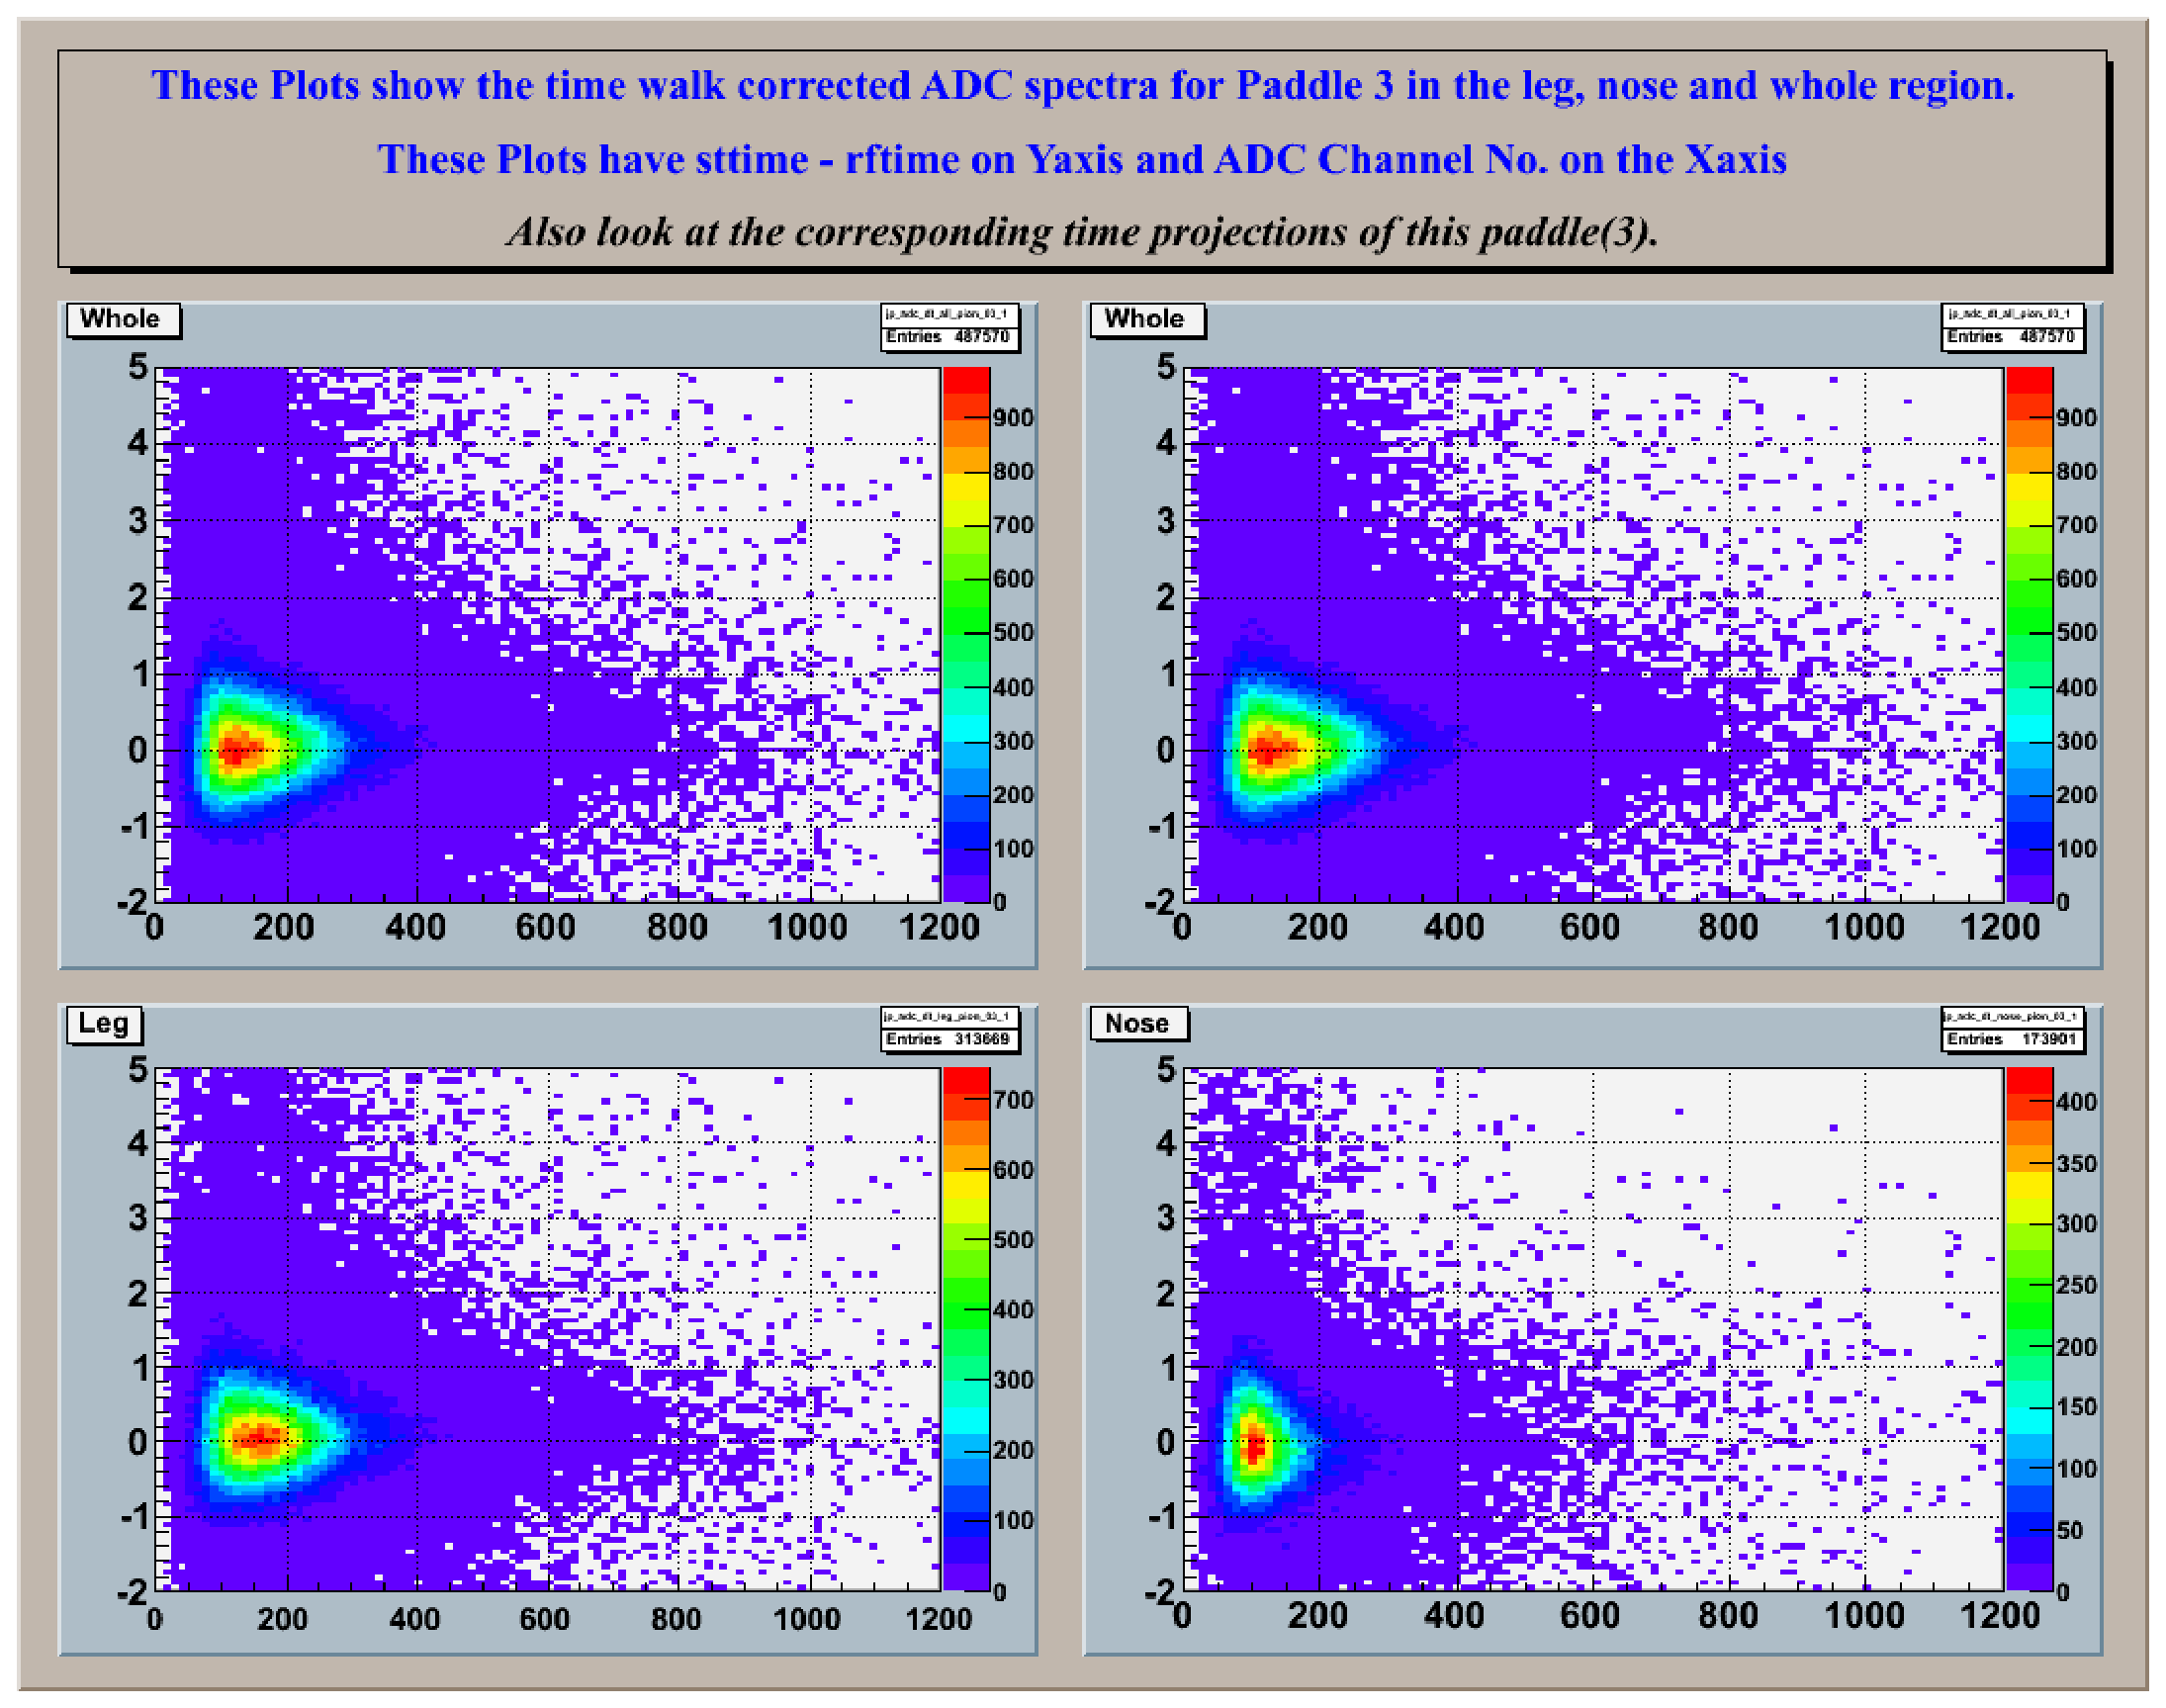
\includegraphics[width=0.65\columnwidth]{figures/calib/st/Corrected_adc.eps}
\caption[]{\label{fig:calib.st.adccor}}
\end{center}\end{figure}

\begin{figure}[htbp]\begin{center}
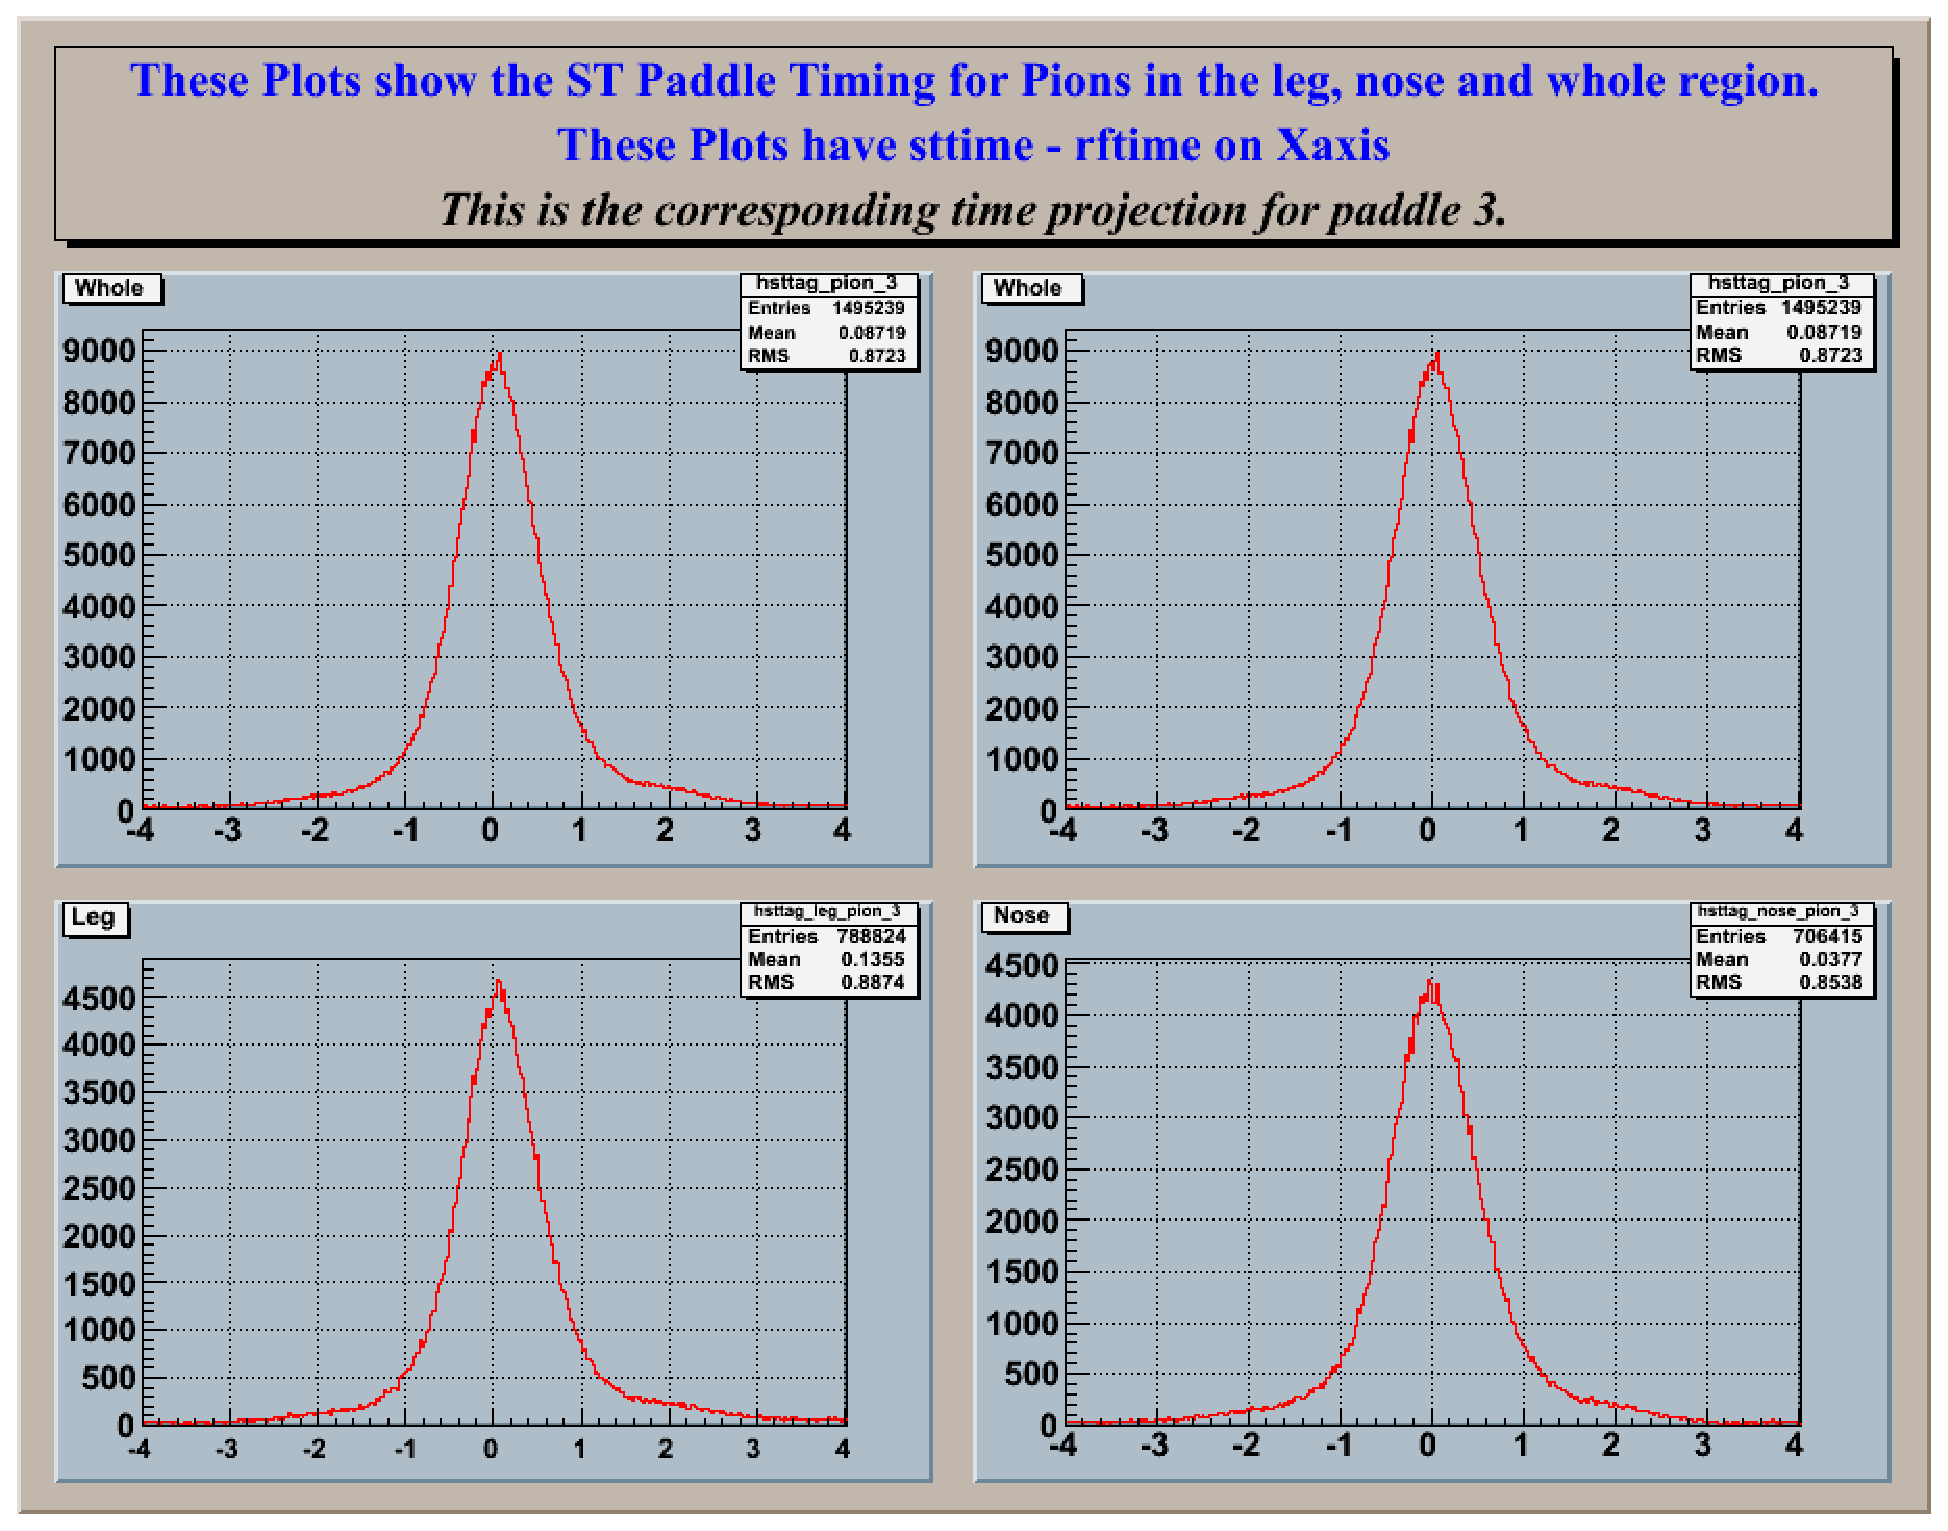
\includegraphics[width=0.65\columnwidth]{figures/calib/st/Hpad3_sttag_pion.eps}
\caption[]{\label{fig:calib.st.timepion}}
\end{center}\end{figure}

\begin{figure}[htbp]\begin{center}
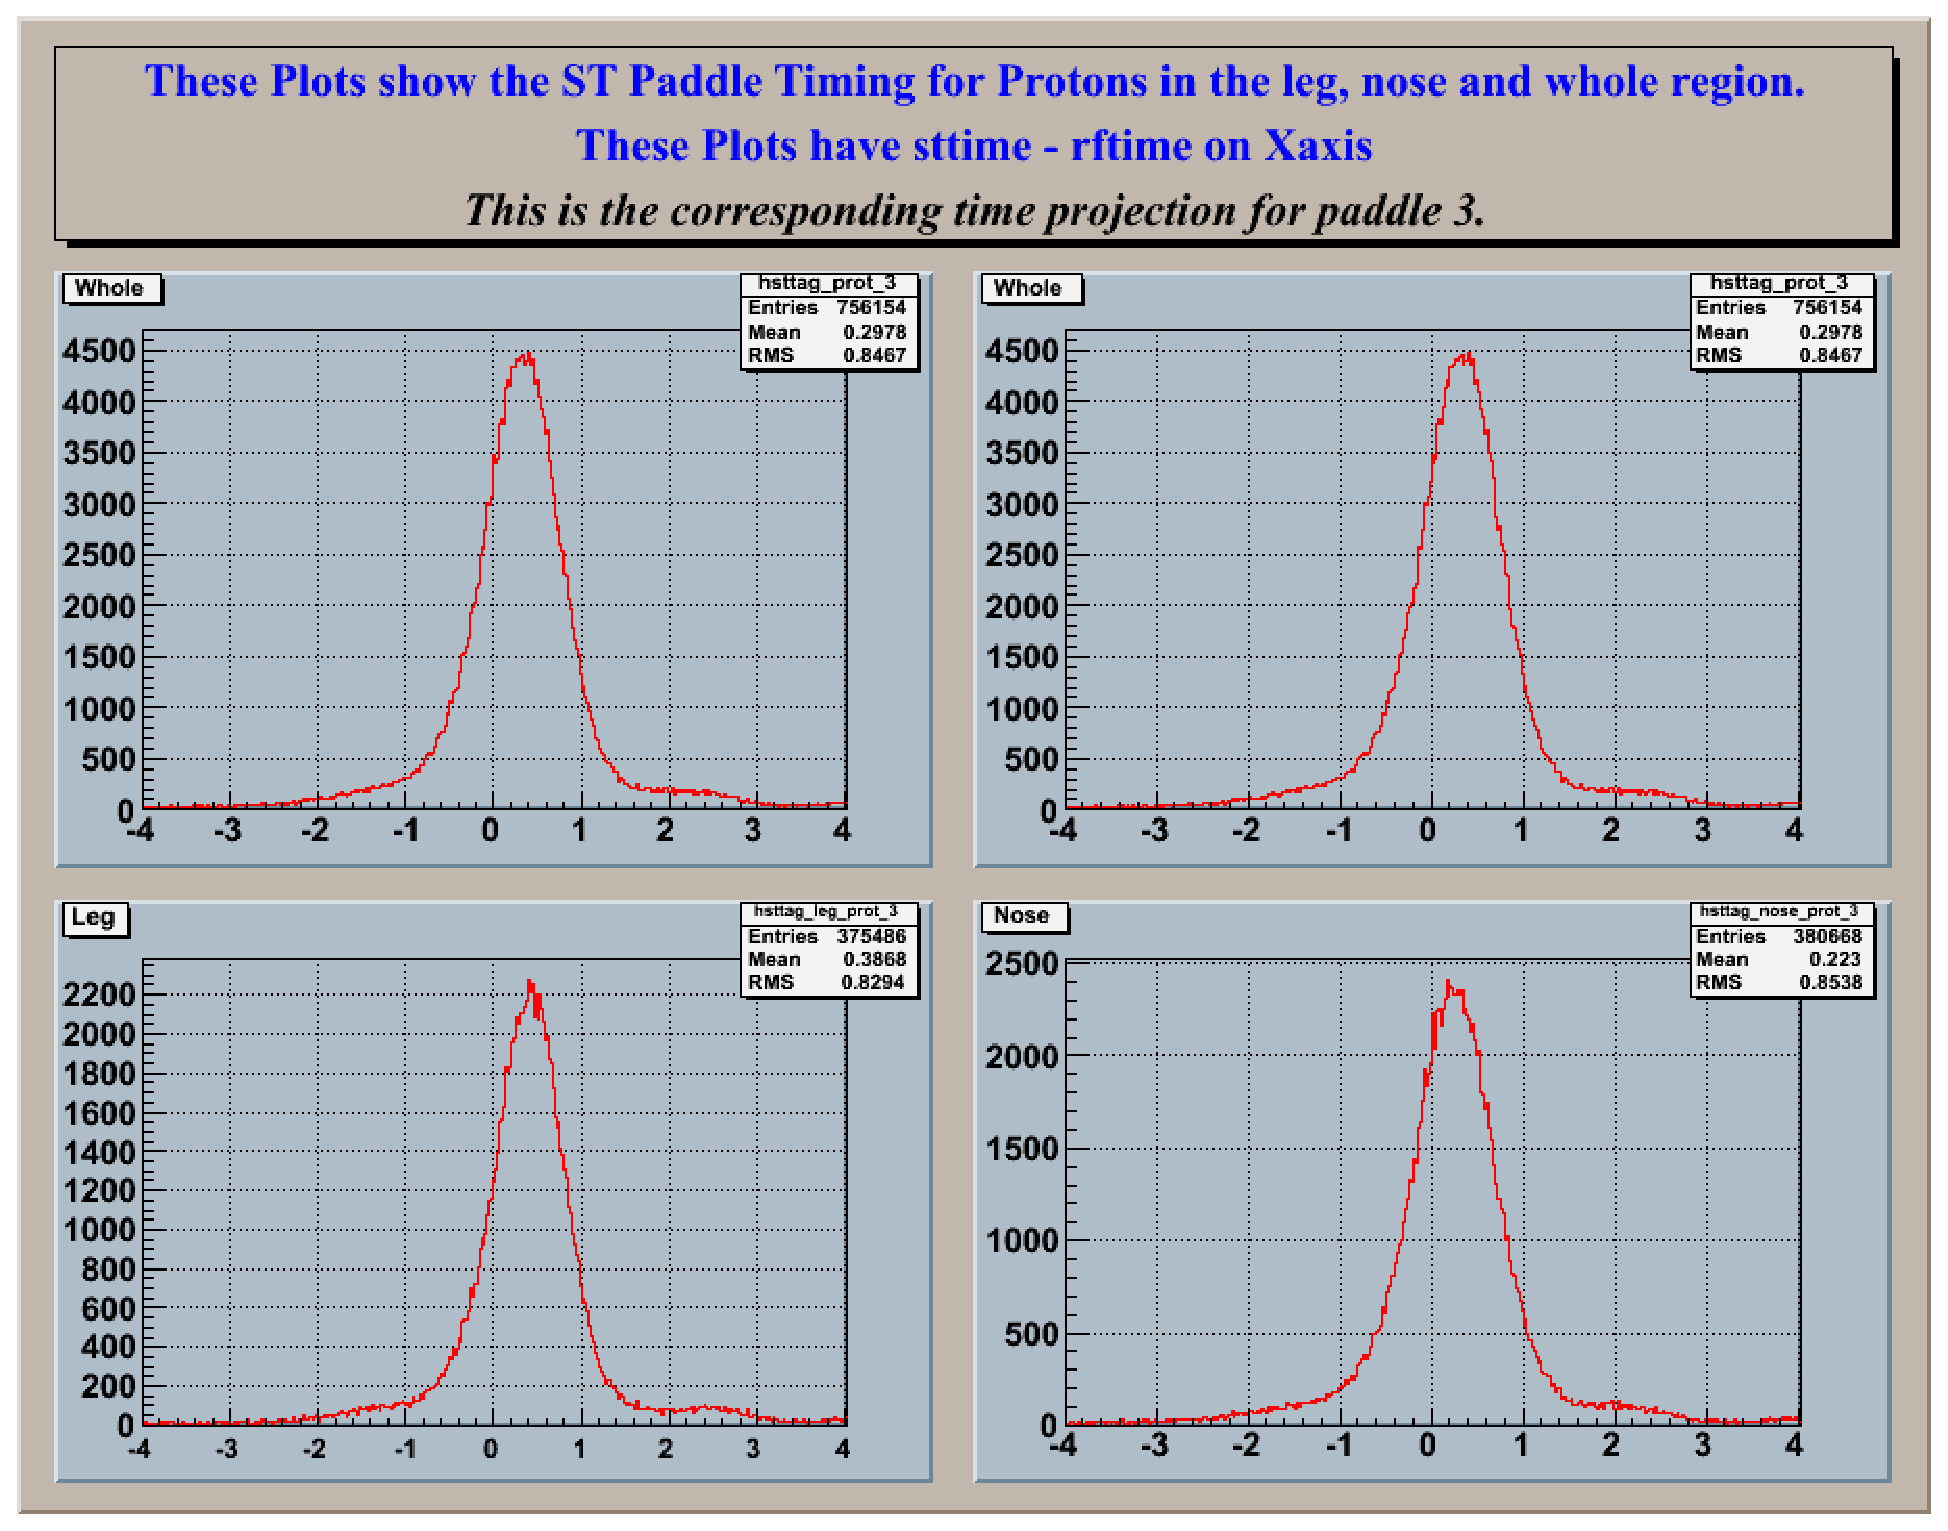
\includegraphics[width=0.65\columnwidth]{figures/calib/st/Hpad3_sttag_prot.eps}
\caption[]{\label{fig:calib.st.timeproton}}
\end{center}\end{figure}

\begin{figure}[htbp]\begin{center}
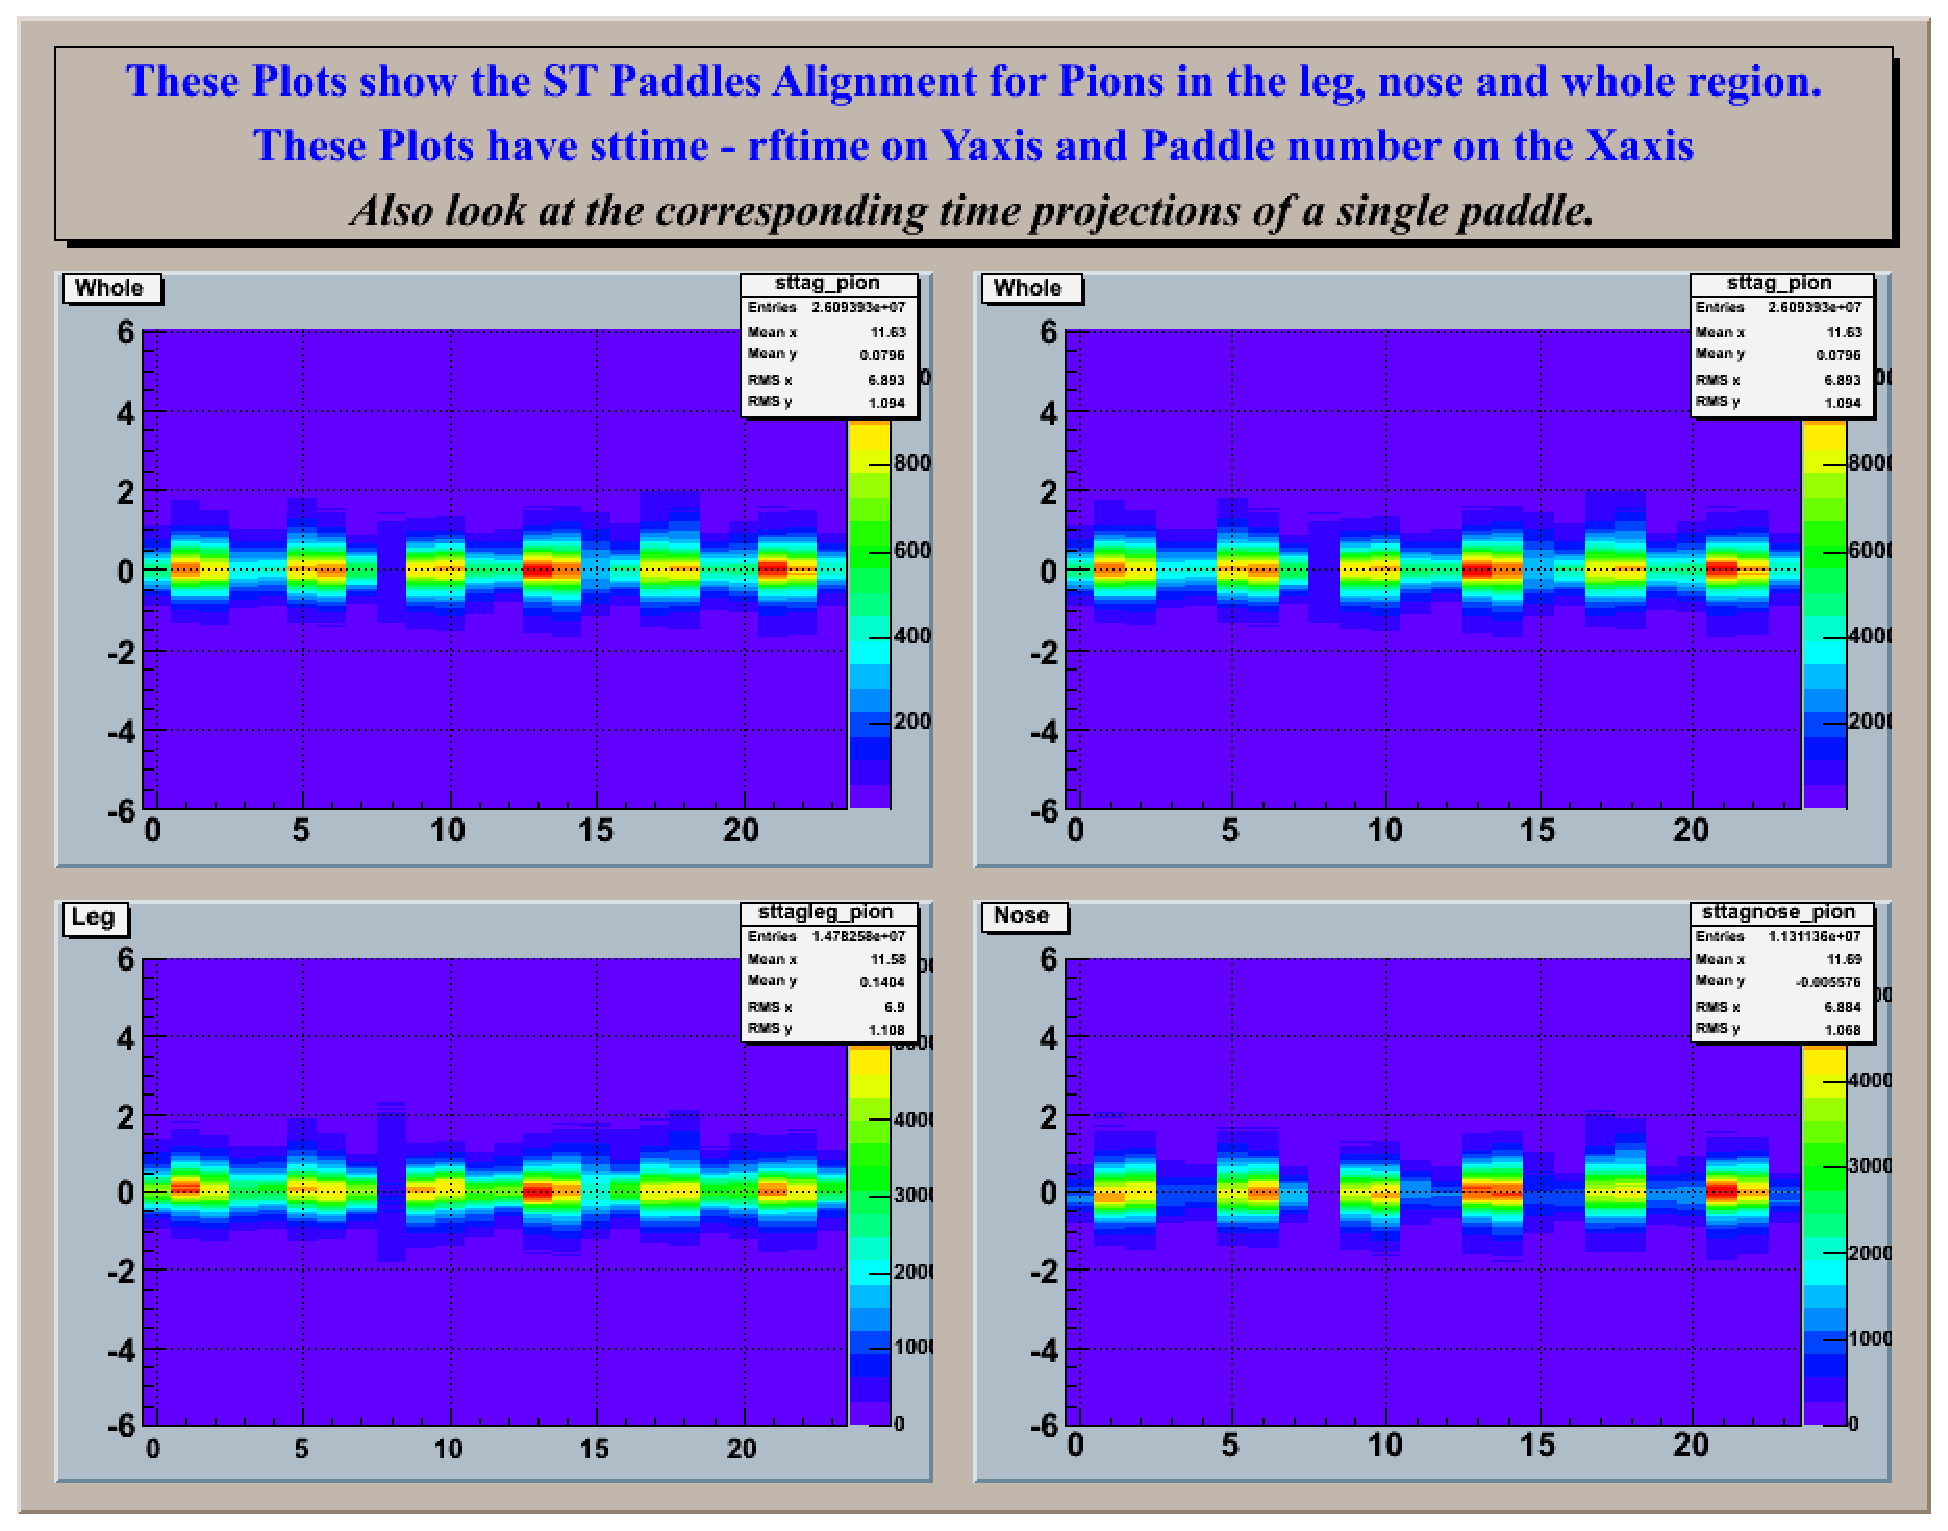
\includegraphics[width=0.6\columnwidth]{figures/calib/st/Hsttag_pion.eps}
\caption[]{\label{fig:calib.st.timepion2d}}
\end{center}\end{figure}

\begin{figure}[htbp]\begin{center}
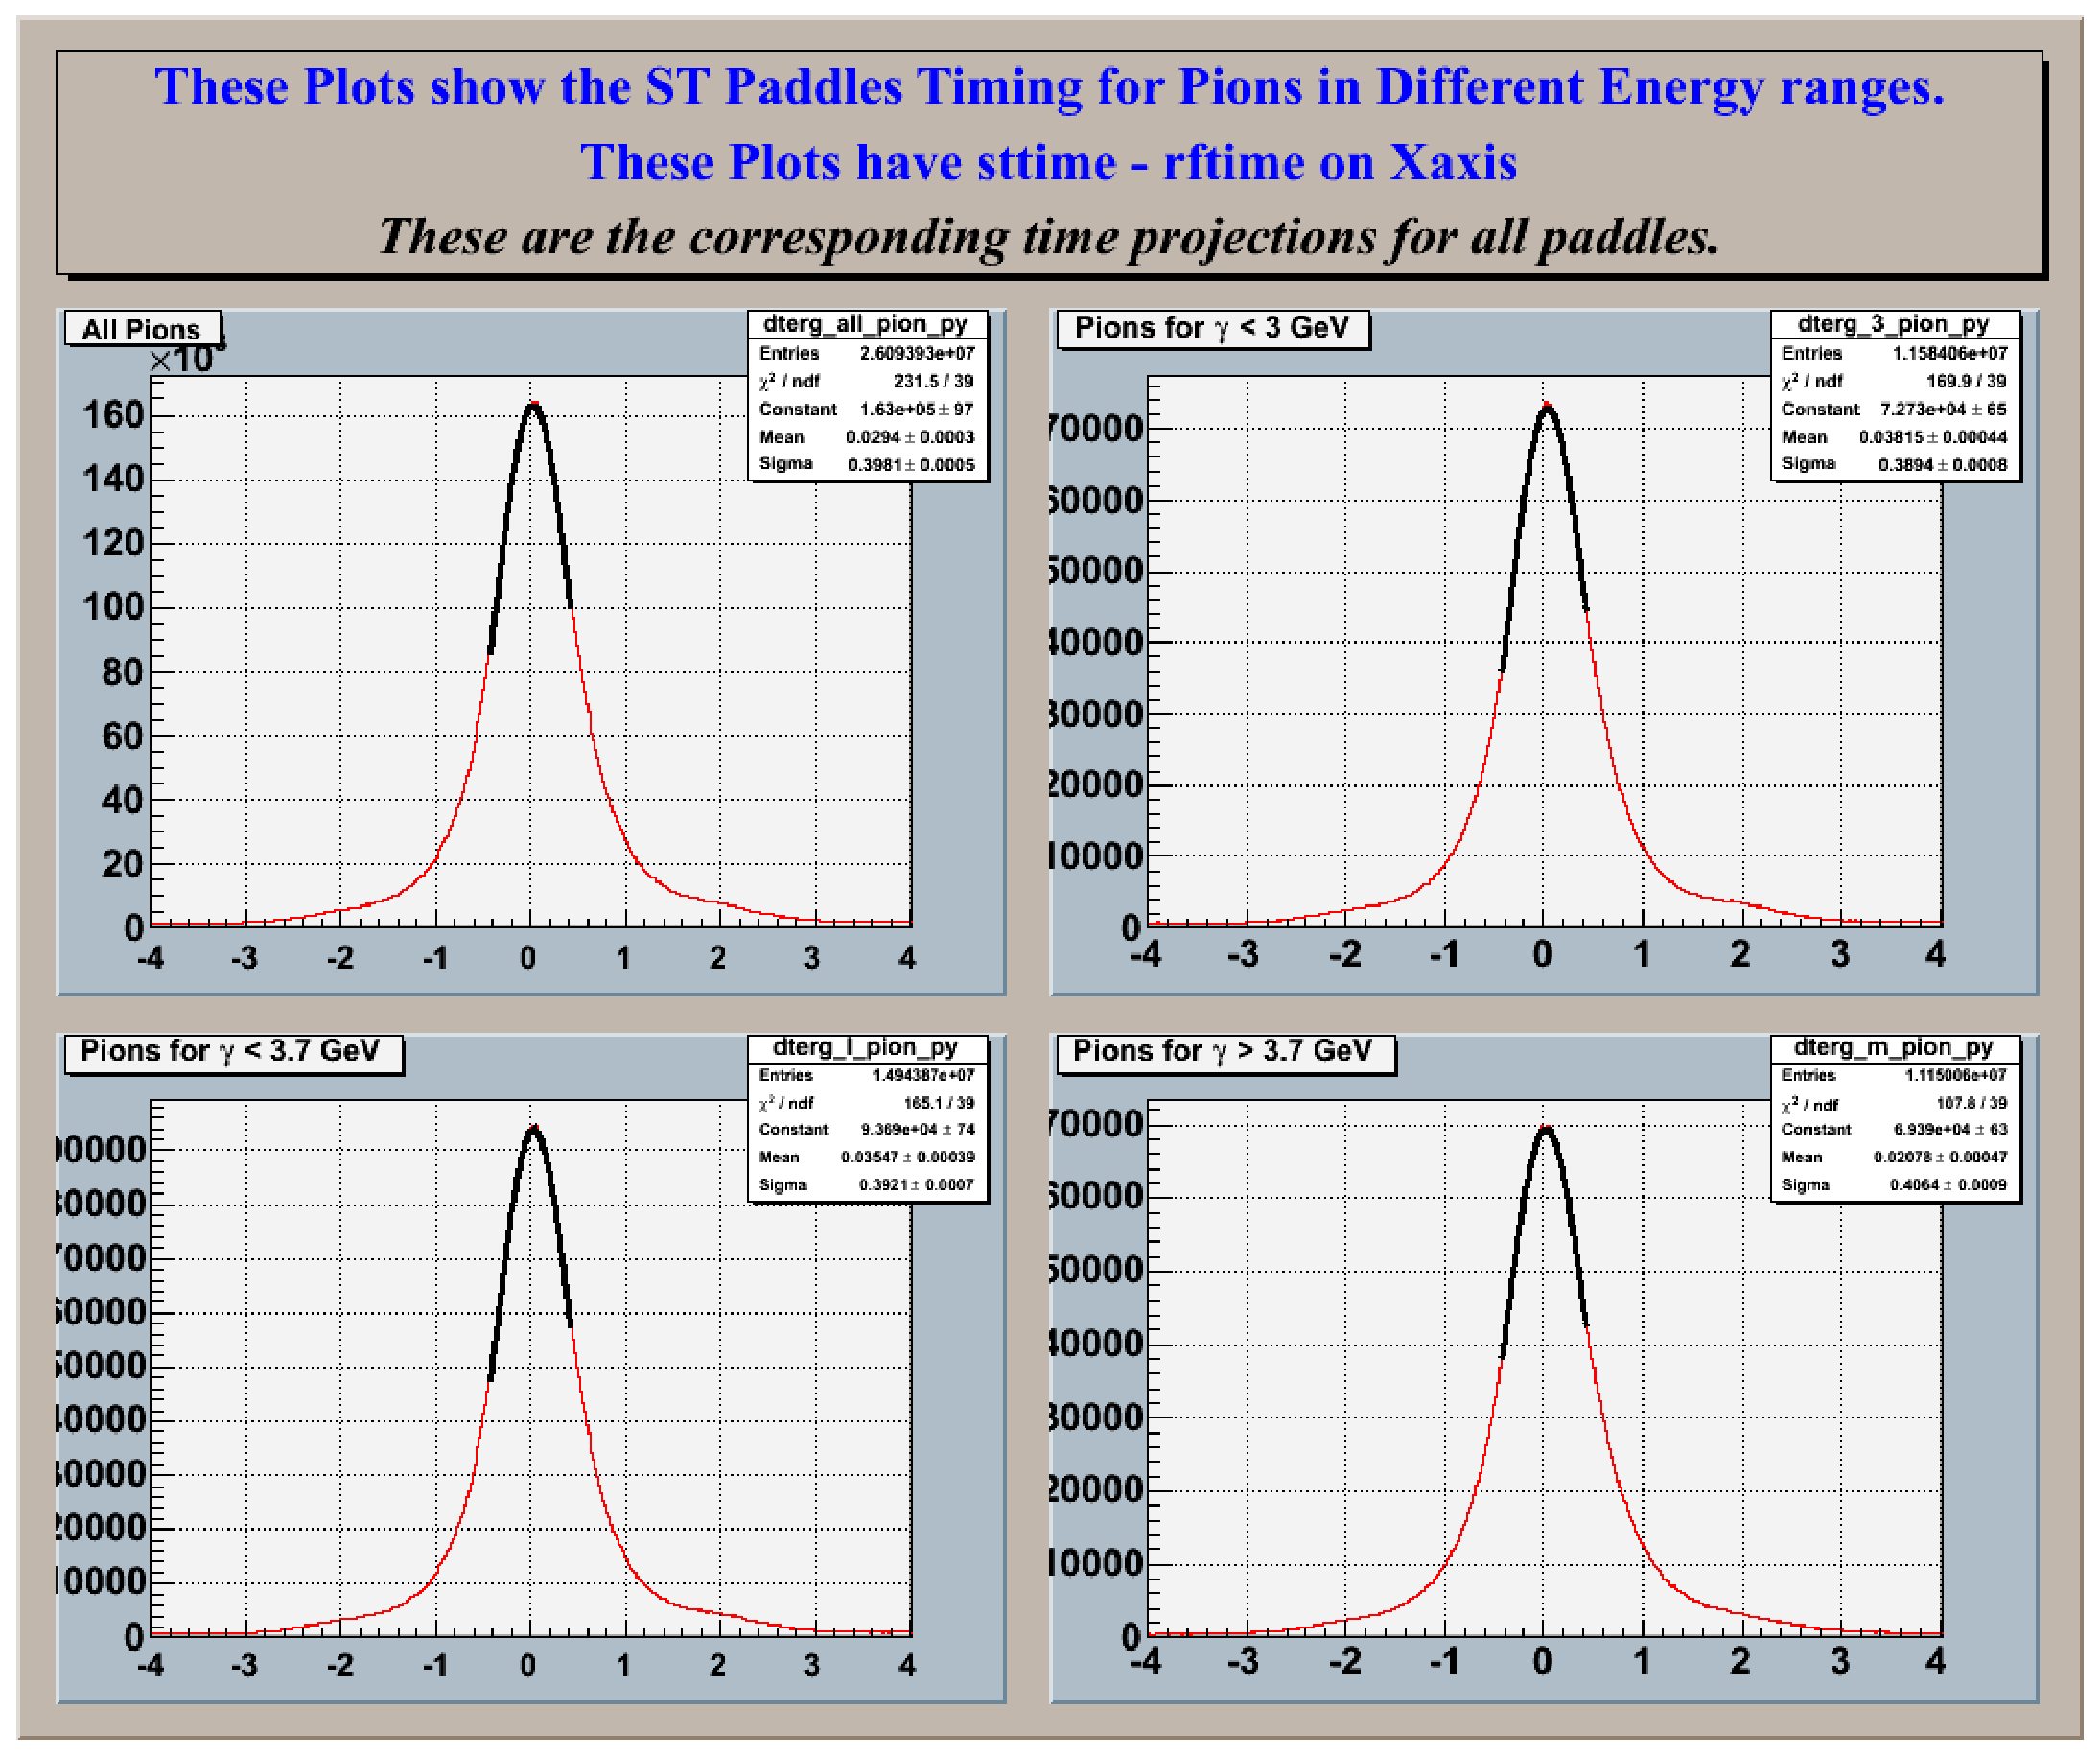
\includegraphics[width=0.6\columnwidth]{figures/calib/st/Sterg_pion.eps}
\caption[]{\label{fig:calib.st.timepion.ebeam}}
\end{center}\end{figure}

\begin{figure}[htbp]\begin{center}
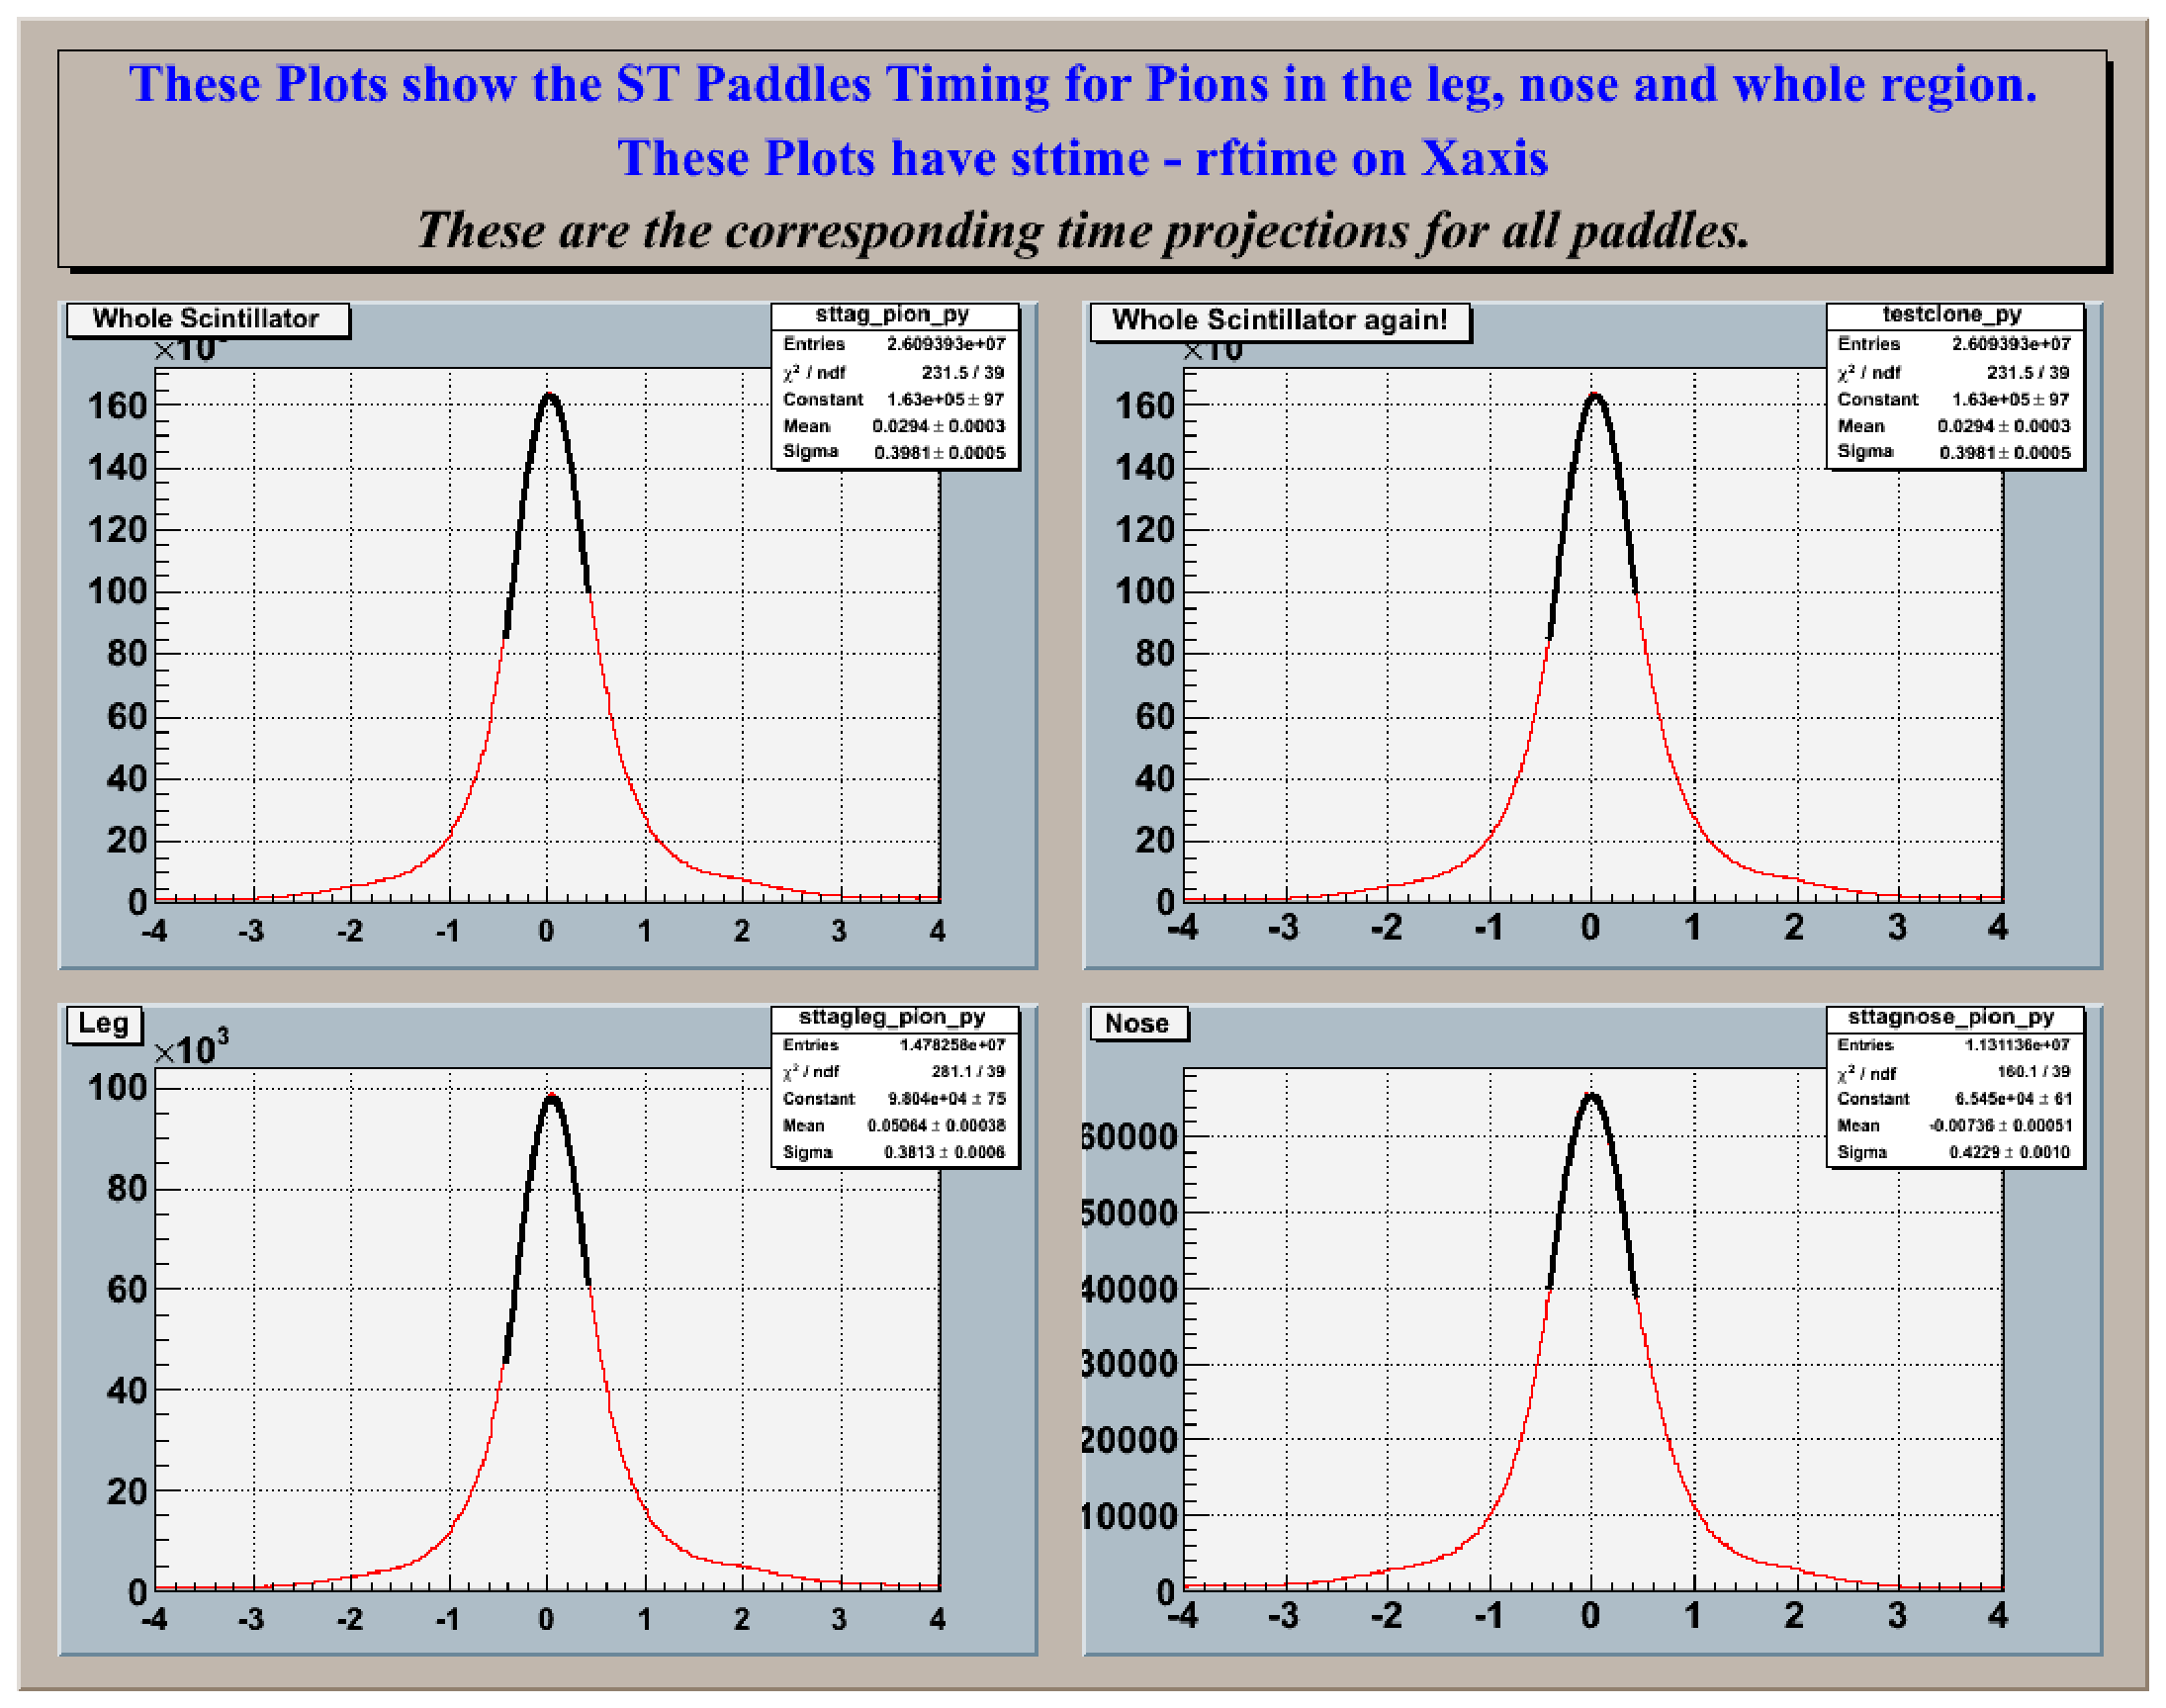
\includegraphics[width=0.6\columnwidth]{figures/calib/st/Timing_pad_3.eps}
\caption[]{\label{fig:calib.st.timepion.region}}
\end{center}\end{figure}

\begin{figure}[htbp]\begin{center}
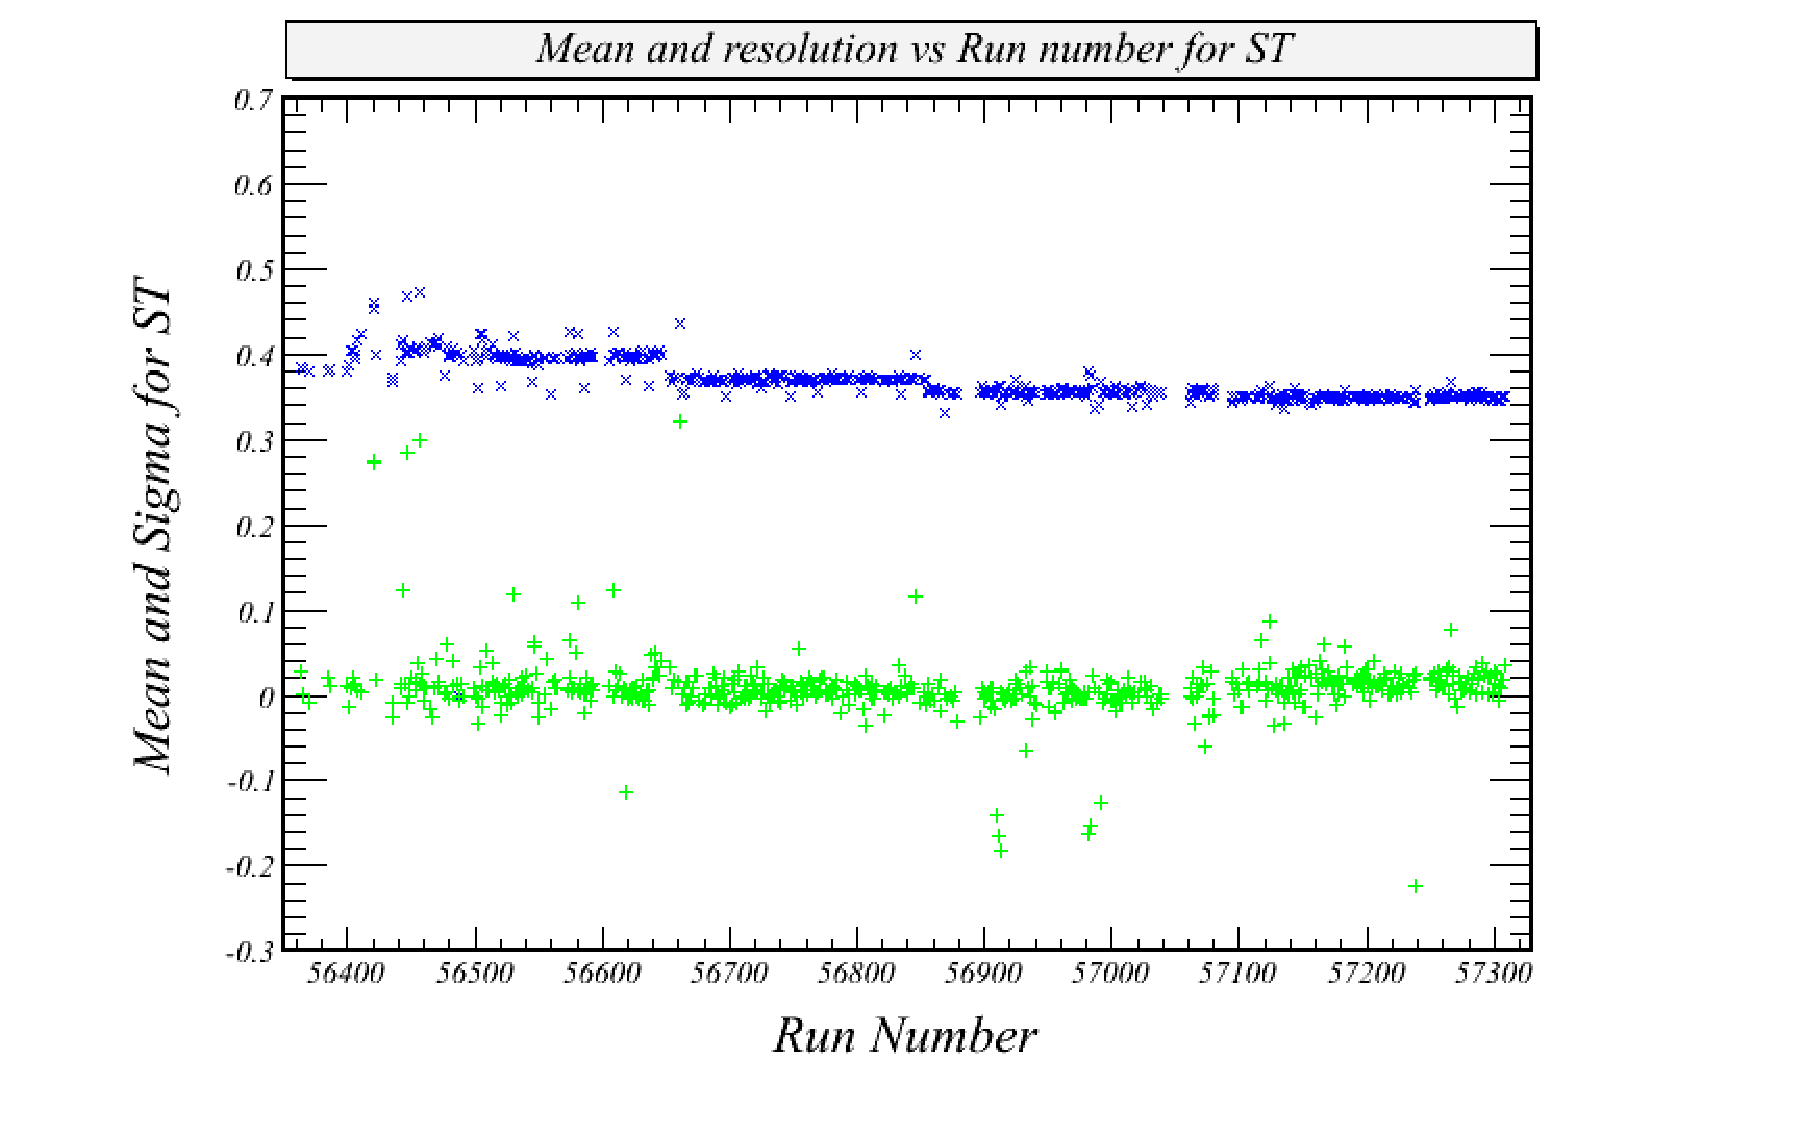
\includegraphics[width=0.65\columnwidth]{figures/calib/st/STmeanandres_v5.eps}
\caption[]{\label{fig:calib.st.runbyrun}}
\end{center}\end{figure}

\FloatBarrier

As a check on the timing resolution of the start counter, we used data containing at least two K$^+$ (this was part of the cascade baryon search) to look at kaons, pion and protons at the same time. The momenta ($p$) of the tracks was given by the drift chamber and tracking algorithm found in the \bank{TBTR} bank, and the energy ($\Epid$) of the particle was set by particle identification. This allowed us to calculate the speed of the particle:
\begin{equation}
    \betapid = \frac{p}{\Epid}.
    \label{eqn:betapid}
\end{equation}
This was used to calculate the vertex time of the particle:
\begin{equation}
    \tvtofpid = \ttof - \frac{\ltof}{c\betapid},
    \label{eqn:tvtofpid}
\end{equation}
where $\ttof$ and $\ltof$ are the time and path length of the track at the \system{TOF} plane as obtained from the \bank{TDPL} bank. This time was converted to a ``photon time'' ($\tpho$) by subtracting the photon propagation time ($\tprop$) from the center of the target:
\begin{equation}
    \tphotofpid = \tvtofpid - \tprop,
    \label{eqn:tphotofpid}
\end{equation}
where
\begin{equation}
    \tprop = \frac{1}{c} \left( \ztgt - \zv \right),
\end{equation}
where $\ztgt$ is the center of the target's z-position ($-90$~cm in the \system{CLAS} coordinate system), and $\zv$ is the z-coordinate of the track's vertex position -- in this case, the intersection of the two kaons where the covariance matrixes of the estimated momenta are taken into account through the standard \prog{MVRT} vertexing algorithm. This photon time, $\tphotofpid$, was compared to the \system{RF}-corrected tagger times ($\ttgrf$) of each hit in the photon tagger as obtained from the \bank{TAGR} bank. The resulting data indicates a timing resolution of 310~ns for protons, 400~ns for pions, and 430~ns for kaons.

\begin{figure}[htbp]\begin{center}
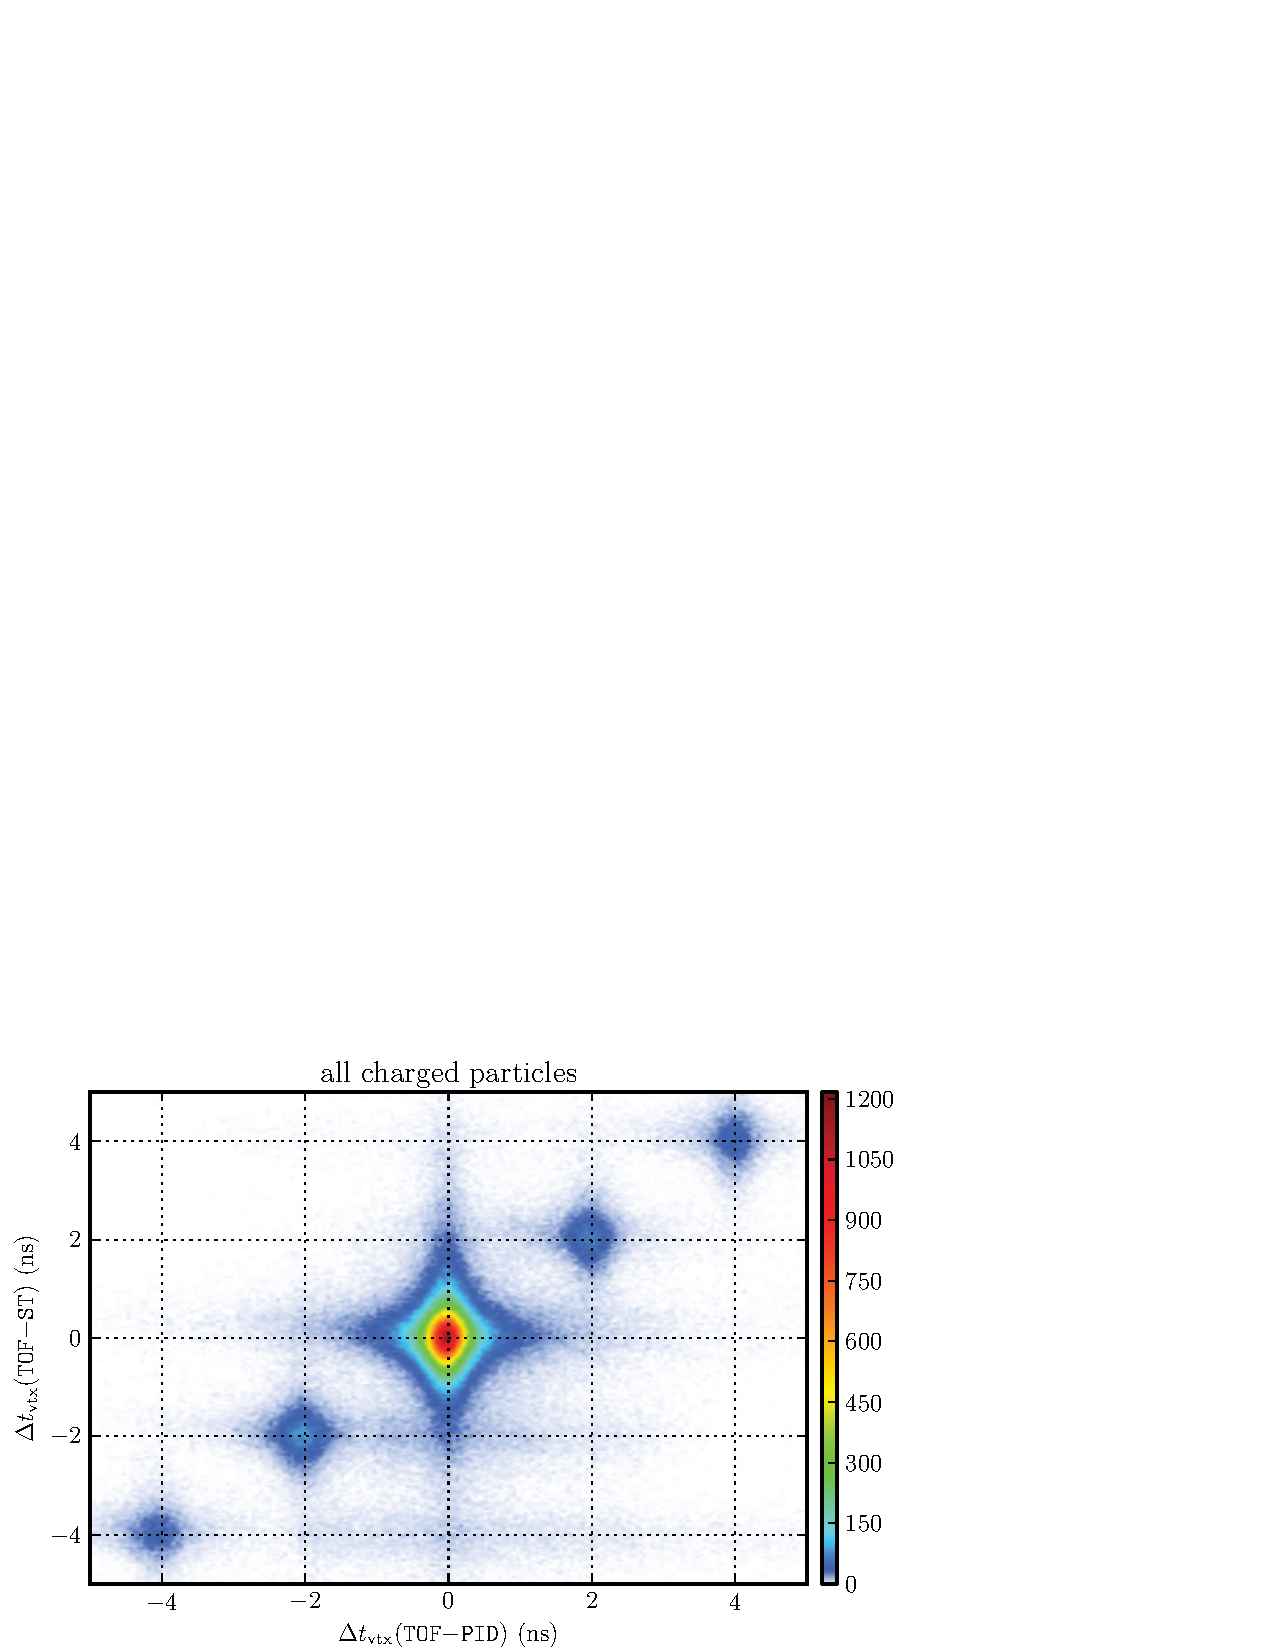
\includegraphics[width=0.5\columnwidth]{figures/calib/st/dvertex_time_pid_st.pdf}
\caption[vertex timing, \abbr{TOF-ST} vs.\ \abbr{TOF-PID}]{\label{fig:dvertex_time_pid_st}Difference in vertex times for each track for the two calculations made above. Represents 1.5\% of the total statistics.}
\end{center}\end{figure}

\begin{figure}[htbp]\begin{center}
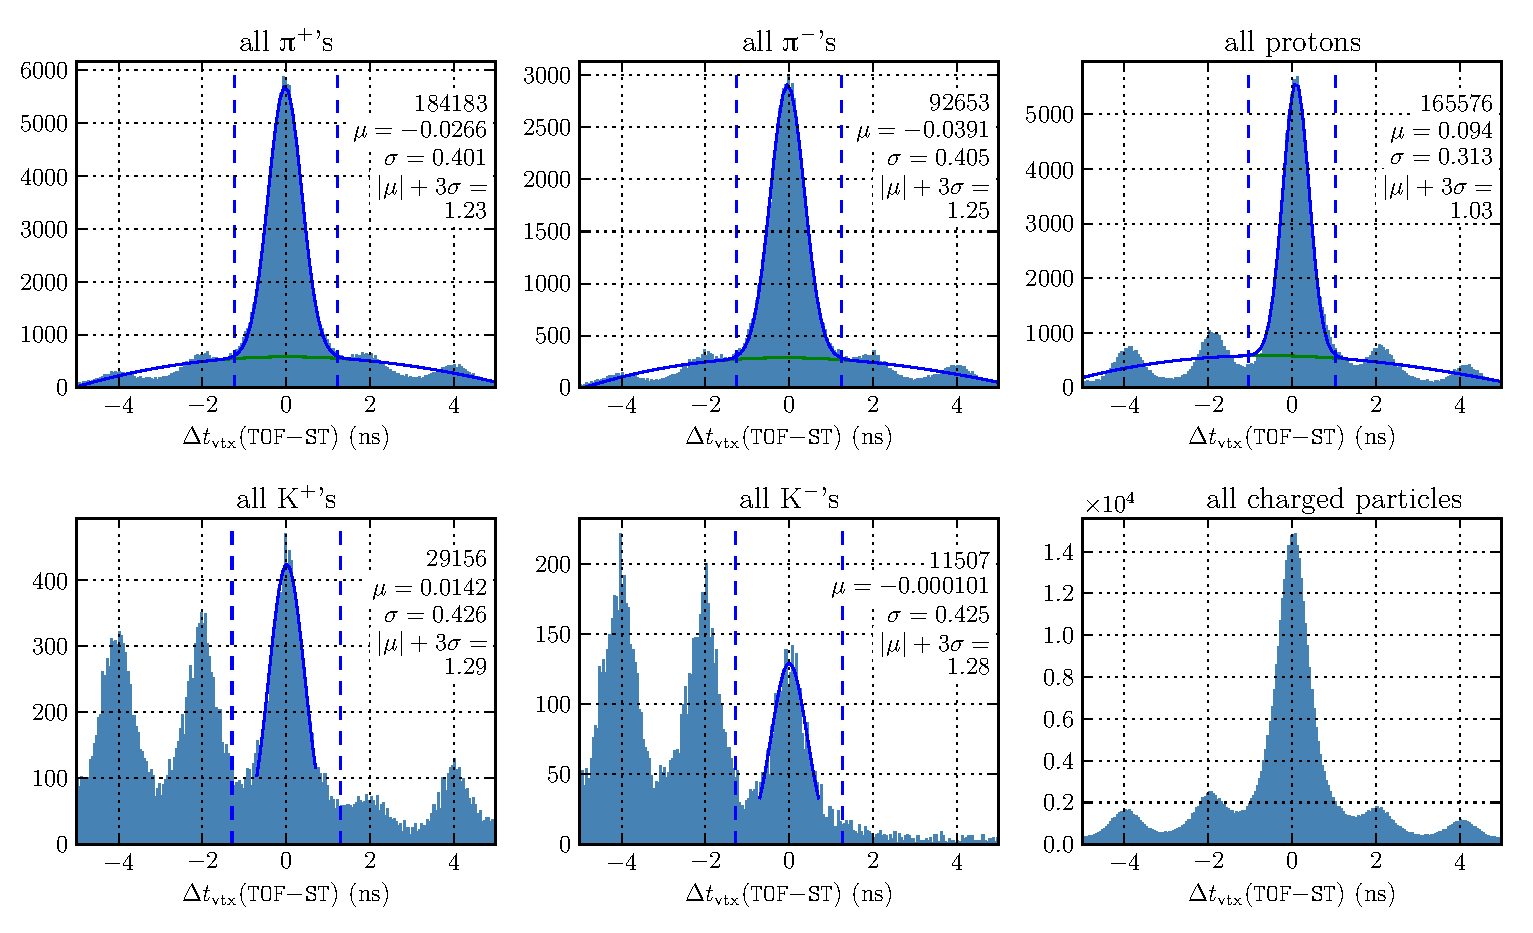
\includegraphics[width=0.9\columnwidth]{figures/calib/st/dvertex_time_st.eps}
\caption[vertex timing, \abbr{TOF-ST}]{\label{fig:dvertex_time_st}Difference in vertex time between that of the photon and of the tracks based on start counter and time-of-flight times. Represents 1.5\% of the total statistics.}
\end{center}\end{figure}


\subsubsection{\label{sec:calib.st.eff}Start Counter Efficiency}

The efficiency of the start counter was calculated by examining the number of tracks with a ST hit after track reconstruction. The ST fired $91.6\%$ of the time, this was calculated from run 57000 since it is a good run and included in production data.

\FloatBarrier
